% chktex-file 3 chktex-file 9 chktex-file 12 chktex-file 17 chktex-file 18 chktex-file 36 chktex-file 40chktex-file 40
\section*{Exercise 12}

Let \(\{X_t\}\) denote the Wölfer sunspot numbers (Example 1.1.5) and let \(\{Y_t\}\) denote the mean-corrected series, \(Y_t = X_t - 46.93, \, t = 1, \ldots, 100\). The following AR(2) model for \(\{Y_t\}\) is obtained by equating the theoretical and sample autocovariances 
at lags 0, 1, and 2:
\[
Y_t - 1.317Y_{t-1} + 0.634Y_{t-2} = Z_t, \quad \{Z_t\} \sim \mathrm{WN}(0, 289.3).
\]
(These estimated parameter values are called "Yule–Walker" estimates and can 
be found using the program PEST, option 3.)
Determine the spectral density of the fitted model and find the frequency at 
which it achieves its maximum value. What is the corresponding period? 
(The spectral density of any ARMA process can be computed numerically using the 
program PEST, option 5.)

\subsection*{Solution}

The spectral density of an ARMA process according to\textbf{ Theorem 4.4.2} is 
\[ f(\lambda) = \frac{\sigma^2}{2\pi} \left| \frac{\theta(e^{-\lambda})}{\phi(e^{-i\lambda})} \right|^2 ,\]
and in our case, $\theta(z) = 1$ and $\psi(z) = 1 - 1.317z-0.634z^2$ with $\sigma^2 = 289.3$ so
\[ f_Y(\lambda) = \frac{289.3}{2\pi} \frac{1}{|1 - 1.317 e^{-i\lambda} - 0.634 e^{-2i\lambda}|^2}. \]
To find $\lambda$ for which $f$ is maximized we must minimize $|1 + a z + v z^2|^2$ for $a = -1.317$, $b = 0.634$ and $z = x+iy$ with the restriction $G(x,y) = |z|^2 = x^2+y^2 = 1$.

\[ F(z) = \left\| \begin{bmatrix}
    1 + ax + bx^2 - by^2\\
    ay + 2bxy
\end{bmatrix} \right\|^2 = (1+ax+bx^2 -by^2)^2 + (ay + 2bxy)^2.
\]
With Lagrange multipliers we obtain that the minimum of this function $F$ at the restriction $G(x,y) = 1$ is
\[ \min_{|z| = 1}F(z) = 0.904401 = (1 - 1.317 - 0.634)^2 \]
at $e^{-i\lambda} = z = 1+0i$, that is when $\lambda = 0$. Thus, 
\[ \max_{\lambda \in [-\pi,\pi]}f(\lambda) = \frac{289.3}{0.904401\cdot 2\pi} \approx 50.9105\]
and the frequency $\lambda$ that maximizes $f$ is $\lambda_{\max} = 0$. Therefore, the period is undefined.

\begin{figure}[H]
    \centering
    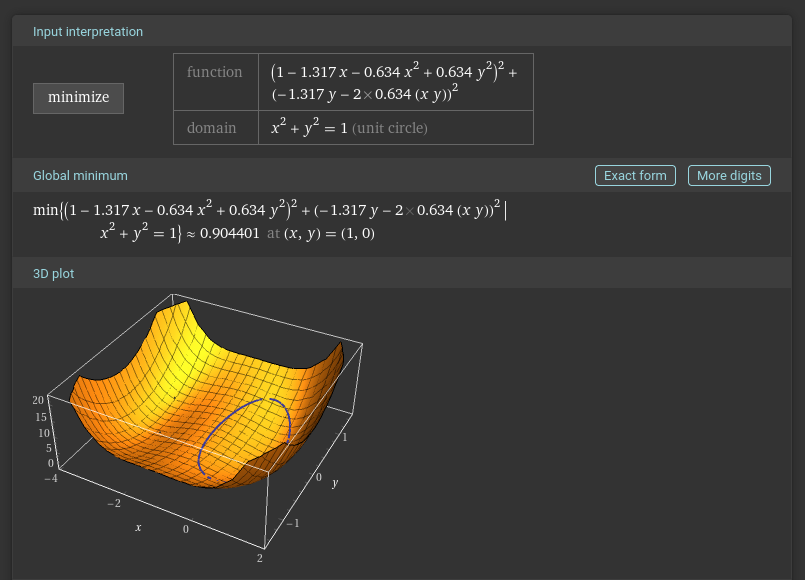
\includegraphics[width=0.85\textwidth]{../pictures/image1.png}
\end{figure}